\section{Spatial Filtering}
\subsection{Task 1: Theory}
\subsubsection*{a)}
Sampling is the process of converting a continuos-time signal to a discrete-time signal, usually by measuring the continuos-time signal at specific points in time and extending this measurement over a set time step. 

\subsubsection*{b)}
Quantization is the process of constraining a signal from a larger to a smaller set of values, like mapping colours to the standard RGB range of 256 integer values. 

\subsubsection*{c)}
A high contrast image histogram would look similar to a dirac delta function, with most values grouped together around the same intensity.

\subsubsection*{d)}


\begin{table}[]
    \label{tab:initial_image}
    I = \begin{tabular}{|l|l|l|l|l|}
        \hline
        5 & 0 & 2 & 3 & 4 \\ \hline
        3 & 2 & 0 & 5 & 6 \\ \hline
        4 & 6 & 1 & 1 & 4 \\ \hline
    \end{tabular}
\end{table}


Couldn't be bothered to do this in Latex, so see \cref{fig:equalizer}. The top matrix is the image before equalization, and the bottom is the image after equalization. The columns are the following: intensities, counts of intensities, pdf, cdf, cdf multiplied with scaling, intensity rounding, new intensity count. Then, using the intensity rounding and mapping the old intensities to the new, we get the final, equalized image. 
\begin{figure}[]
    \centering
    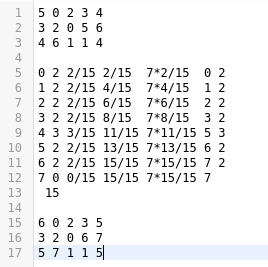
\includegraphics[width=1.00\textwidth]{figures/histogram_equalizer.png}
    \caption{Histogram equalization}
    \label{fig:equalizer}
\end{figure}

\subsubsection*{e)}
The log transform will increase the output intensity for low input intensities, and flatten for high input intensities. This will make it easier to see the lower ranges of the input intensities. If we then apply this transform to a high variance image, then the lower part of the dynamic range will be enhanced, while the higher part looses information. 
%
% SOMETHING MORE 
%
%

\subsubsection*{f)}
\begin{table}[]
    \label{tab:kernel}
    K = \begin{tabular}{|l|l|l|l|l|}
        \hline
        0 & 0 & 0 \\ \hline
        1 &-4 & 1 \\ \hline
        0 & 1 & 0 \\ \hline
    \end{tabular}
\end{table}

Using zero-padding for this convolution. I flipped the kernel and used correlation and matrix multiplication to get the convolution. Convolving \cref{tab:initial_image} and \cref{tab:kernel}. See \cref{tab:kernel_convolution}: 
\begin{table}[]
    \label{tab:kernel_convolution}
    \begin{tabular}{|l|l|l|l|l|}
        \hline
        -17 & 9 & -4 & -4 & -10 \\ \hline
        -1 & 1 & 10 & -9 & -10 \\ \hline 
        -7 & -17 & 3 & 6 & -9 \\ \hline
    \end{tabular} 
\end{table}

\newpage
\subsection{Task 2: Programming}
\subsubsection*{a)}
See the result from \cref{fig:greyscale}. 
\begin{figure}[]
    \centering
    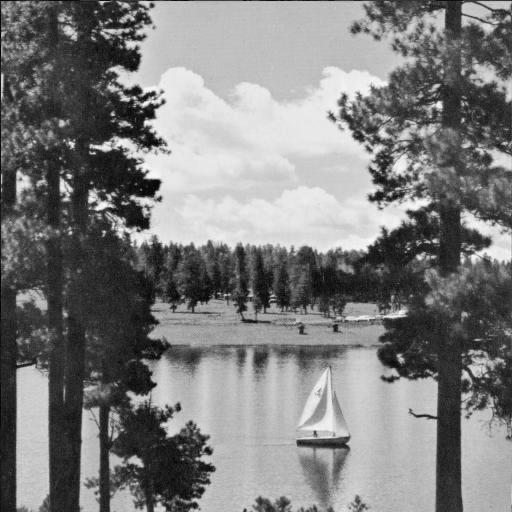
\includegraphics[width=1.00\textwidth]{figures/image_processed/lake_greyscale.jpg}
    \caption{The grey scale version of the lake image}
    \label{fig:greyscale}
\end{figure}

\subsubsection*{b)}
Se the result from \cref{fig:inverse}. 
\begin{figure}[]
    \centering
    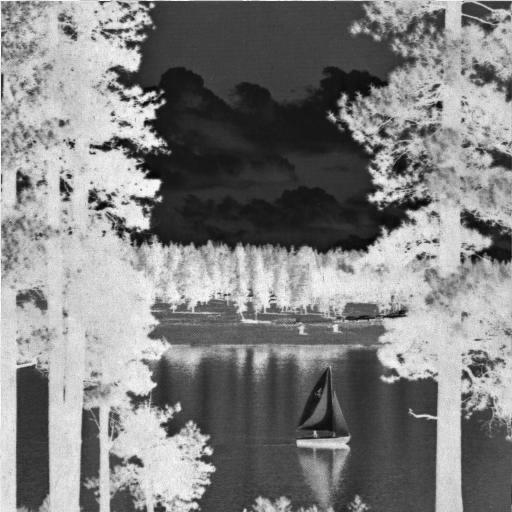
\includegraphics[width=1.00\textwidth]{figures/image_processed/lake_inverse.jpg}
    \caption{The inverse of the grey scale version of the lake image}
    \label{fig:inverse}
\end{figure}

\subsubsection*{c)}
See the results from \cref{fig:convolution_h_a} and \cref{fig:convolution_h_b}.

\begin{figure}[]
    \centering
    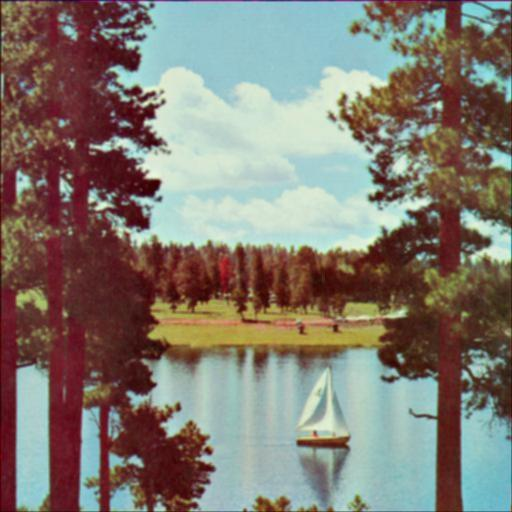
\includegraphics[width=1.00\textwidth]{figures/image_processed/convolved_im_h_a.jpg}
    \caption{Convolution of the lake image with the kernel $h_a$.}
    \label{fig:convolution_h_a}
\end{figure}

\begin{figure}[]
    \centering
    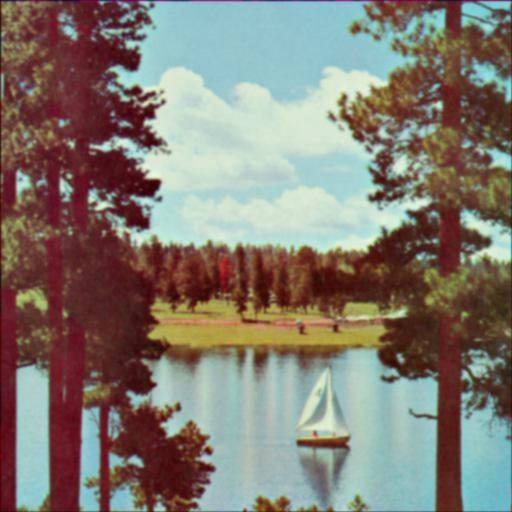
\includegraphics[width=1.00\textwidth]{figures/image_processed/convolved_im_h_b.jpg}
    \caption{Convolution of the lake image with the kernel $h_b$.}
    \label{fig:convolution_h_b}
\end{figure}
